% Created 2022-07-25 월 10:11
% Intended LaTeX compiler: pdflatex
\documentclass[11pt]{article}
\usepackage[utf8]{inputenc}
\usepackage[T1]{fontenc}
\usepackage{graphicx}
\usepackage{longtable}
\usepackage{wrapfig}
\usepackage{rotating}
\usepackage[normalem]{ulem}
\usepackage{amsmath}
\usepackage{amssymb}
\usepackage{capt-of}
\usepackage{hyperref}
\documentclass[10pt, twoside, a4paper]{slides}
\usepackage[landscape, fleqn]{geometry}
\usepackage{blindtext, fancyhdr}
\usepackage{kotex}
\usepackage{lmodern}
\usepackage[utf8]{inputenc}
\usepackage{graphicx}
\usepackage{amsmath, amsthm, amssymb}
\usepackage[table, xcdraw]{xcolor}
\usepackage{listings}
\author{syryu}
\date{\today}
\title{}
\hypersetup{
 pdfauthor={syryu},
 pdftitle={},
 pdfkeywords={},
 pdfsubject={},
 pdfcreator={Emacs 28.1 (Org mode 9.5.2)},
 pdflang={English}}
\begin{document}

\tableofcontents


\section{Vi mode (default control)}
\label{sec:org0ce81b0}
\begin{center}
\begin{tabular}{llll}
esc & i & v & :\\
\hline
default 상태 & 입력모드 & 선택모드 & 명령어모드\\
l(or right) 한 칸 이동 & 키보드 입력 & esc와 동일 & :w 저장\\
h(or left) 한 칸 뒤로 이동 &  & esc와 동일 & :q 끝내기\\
j(or down) 아래로 한 줄 이동 &  & esc와 동일 & :wq or :x 저장 후 끝내기\\
k(or up) 위로 한 줄 이동 &  & esc와 동일 & :q! 강제 종료\\
w(or e) 한 단어 앞으로 이동 &  & esc와 동일 & :w /path/file\_name 다른이름으로 저장\\
b 한 단어 뒤로 이동 &  & esc와 동일 & \\
) 한 문장 앞으로 이동 &  & esc와 동일 & \\
\} 한 문단 앞으로 이동 &  & esc와 동일 & \\
y 선택영역 복사 &  & esc와 동일 & \\
yy 한 줄 복사 &  & yy 없음 & \\
p 붙여넣기 &  & esc와 동일 & \\
d 선택영역 잘라내기 &  & esc와 동일 & \\
dd 한 줄 잘라내기 &  & dd 없음 & \\
u 실행 취소(undo) &  & esc와 동일 & \\
ctrl-r 다시 실행(redo) &  & esc와 동일 & \\
ctrl-h t 테마설정(nova) &  &  & \\
\end{tabular}
\end{center}
\section{Windows (spc w)}
\label{sec:org0846ee3}
\begin{center}
\begin{tabular}{lllllllll}
새로 생성 & s & v & n &  &  &  &  & \\
창 이동 & h & j & k & l & b & t & r & R\\
배열 변경 & H & J & K & L &  &  &  & \\
크기 조정 & = & \_ & shift-$\backslash$ & o &  &  &  & \\
창 닫기 & c & d & q &  &  &  &  & \\
\end{tabular}
\end{center}
\section{work space (spc TAB)}
\label{sec:org9658dc1}
\section{Buffer (spc b)}
\label{sec:orgd457401}
\begin{center}
\begin{tabular}{llllll}
버퍼이동 & [ or p & ] or n & b 목록에서 선택 & B b의 확장판 & l 마지막 버퍼\\
버퍼생성/킬 & C 새창에 복사 & d 현재 버퍼 킬 & K 모든 버퍼 킬 & O 현재 버퍼 제외 올 킬 & s 현재 버퍼 저장\\
spc b i (목록) & m 마크 & u 언마크 & t 모든 버퍼 마크 & D  선택된 버퍼 킬 & q 나가기\\
\end{tabular}
\end{center}
\section{Dired mode(spc .)}
\label{sec:org278f5fa}
\begin{center}
\begin{tabular}{lllll}
\^{} 한 단계 위로 & + 새 폴더 만들기 & R 이름 변경 , 경로 지정 & m 마크 & u 언마크\\
d 지우기 마크 & x 지우기 마크된 파일/폴더 지우기 & D 바로 지우기 & M 이동 모드 & C 다른이름으로 저장\\
\end{tabular}
\end{center}
\section{Command(M x or spc :)}
\label{sec:org09842a3}
\begin{center}
\begin{tabular}{lll}
ansi-term & term & shell\\
터미널 위치에서 'spc o -' 현재 위치가 dired mode로 열림 &  & \\
\end{tabular}
\end{center}
\section{magit (spc g)}
\label{sec:org1108879}
\subsection{basic command}
\label{sec:org66f527c}
\begin{center}
\begin{tabular}{ll}
'g' = git status & '/' or 'g C-c C-c'  dispatch mode\\
\end{tabular}
\end{center}
\subsection{시작(remote-repository를 local에 복사, git clone)}
\label{sec:orgd4ccf30}
\begin{center}
\begin{tabular}{ll}
dired mode에서 상위 폴더에 위치 (home/git\_test/를 연동시키려면 home/에 위치) & 'C u url주소(C-v로 가능)' =  git clone <url>\\
\end{tabular}
\end{center}
\subsection{시작( local을 remote-repository에 복사, git init)}
\label{sec:org3fe2962}
\begin{center}
\begin{tabular}{ll}
dired mode에서 원하는 폴더에 위치 (home/git\_test/를 연동시키려면 home/git\_test에 위치) & '/ I' = git init\\
'/ M a' = git remote add <Remote name> <url> & \\
\end{tabular}
\end{center}
\subsection{staging(git add)}
\label{sec:org4263d36}
\begin{center}
\begin{tabular}{ll}
'g s' = 선택항목 staging & 'g S'= 전체변경사항 staging\\
\end{tabular}
\end{center}
\subsection{commit(git commit -m)}
\label{sec:orgd9ac640}
\begin{center}
\begin{tabular}{l}
'g C-c C-c c c <메세지> C-c C-c'\\
\end{tabular}
\end{center}
\subsection{push(git push)}
\label{sec:orgfd7f4ed}
\begin{center}
\begin{tabular}{l}
'g C-c C-c P u' or 'spc g / P u'\\
\end{tabular}
\end{center}

\begin{center}
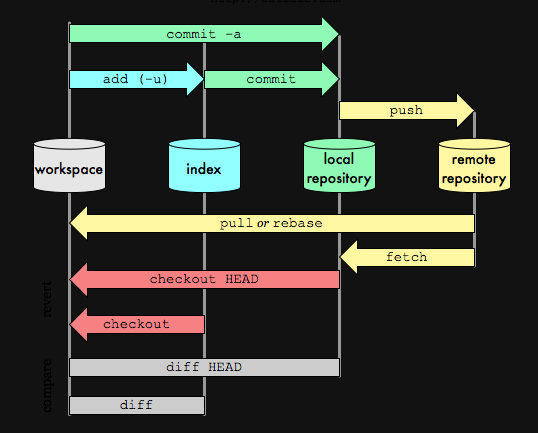
\includegraphics[width=.9\linewidth]{./img/git_structure.png}
\label{fig:1}
\end{center}
\begin{center}
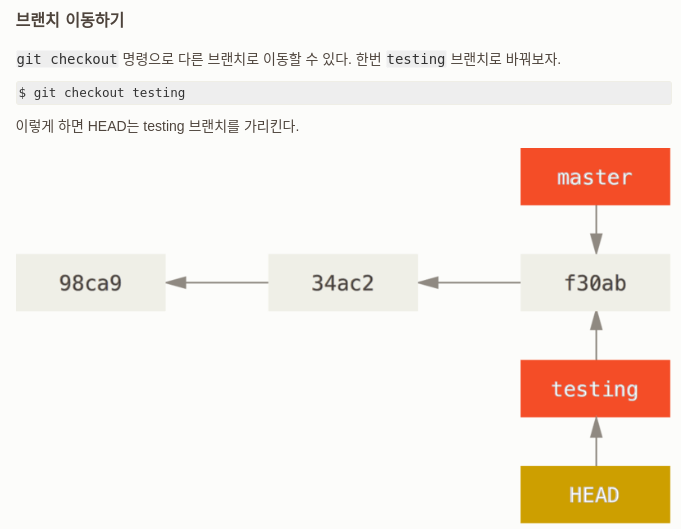
\includegraphics[width=.9\linewidth]{./img/branch_structure.png}
\label{fig:2}
\end{center}

\url{https://velog.io/@csy9604/\%EA\%B8\%B0\%EB\%B3\%B8-\%EA\%B0\%9C\%EB\%85\%90-\%EC\%A0\%95\%EB\%A6\%AC}
\url{https://git-scm.com/book/ko/v2/Git\%EC\%9D\%98-\%EA\%B8\%B0\%EC\%B4\%88-Git-\%EC\%A0\%80\%EC\%9E\%A5\%EC\%86\%8C-\%EB\%A7\%8C\%EB\%93\%A4\%EA\%B8\%B0}
\section{org mode}
\label{sec:orgbce0be9}
\begin{center}
\begin{tabular}{ll}
C-c C-e 파일 extract & * TAB 헤드 타이틀 생성\\
\end{tabular}
\end{center}
\end{document}
